\section{Results}

In this section we present the results of the experiments explained in \ref{ssec:experiments}. Figures~\ref{fig:sir_plots} and~\ref{fig:sis_plots} show the variaton of infected and recovered hosts ($y$ axis) over the time ($x$ axis). Black and green lines represent the average variation of infected and recovered number of hosts (respectively) over time for each network type. Red and blue dashed lines represent the variation of infected nodes over the time in the network with the higher and lower peak (respectively) of infected hosts. Figure~\ref{fig:sir_plots} is the result of the experiments for the SIR epidemics and figure~\ref{fig:sis_plots} for the SIS.

\begin{figure*}[hbtp]
    \centering
    \begin{subfigure}[b]{0.45\textwidth}
        \centering
          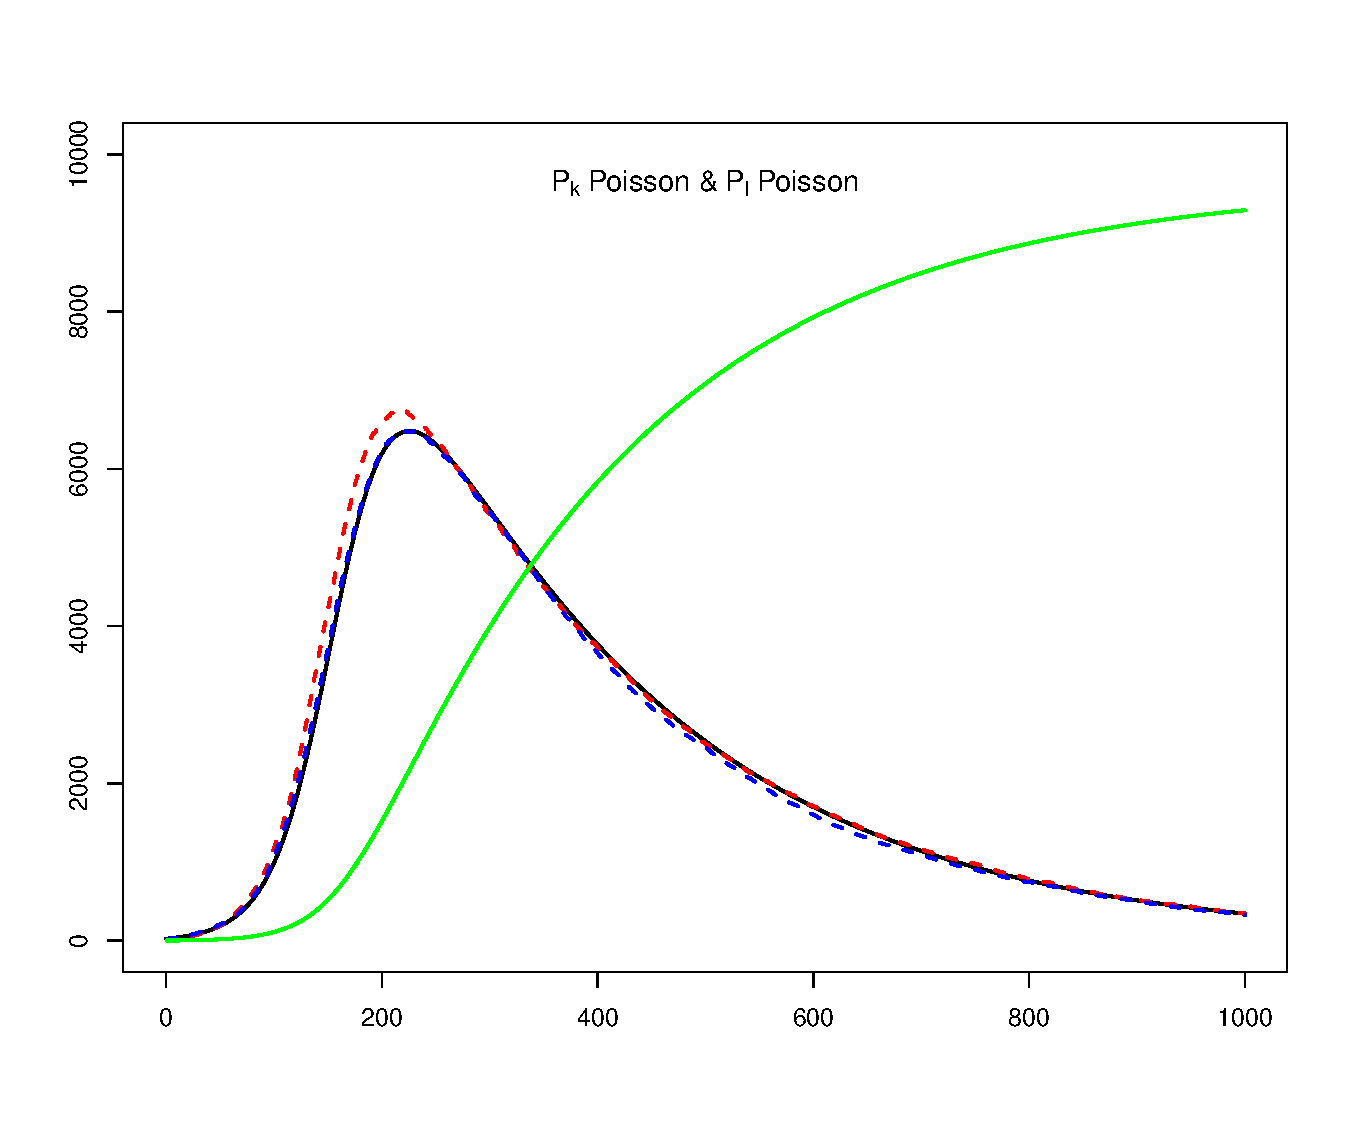
\includegraphics[width=\textwidth, trim=30 20 30 20, clip]{../img/sir_00.pdf}
    \end{subfigure}
    \hspace{0.08\textwidth}
    \begin{subfigure}[b]{0.45\textwidth}
        \centering
          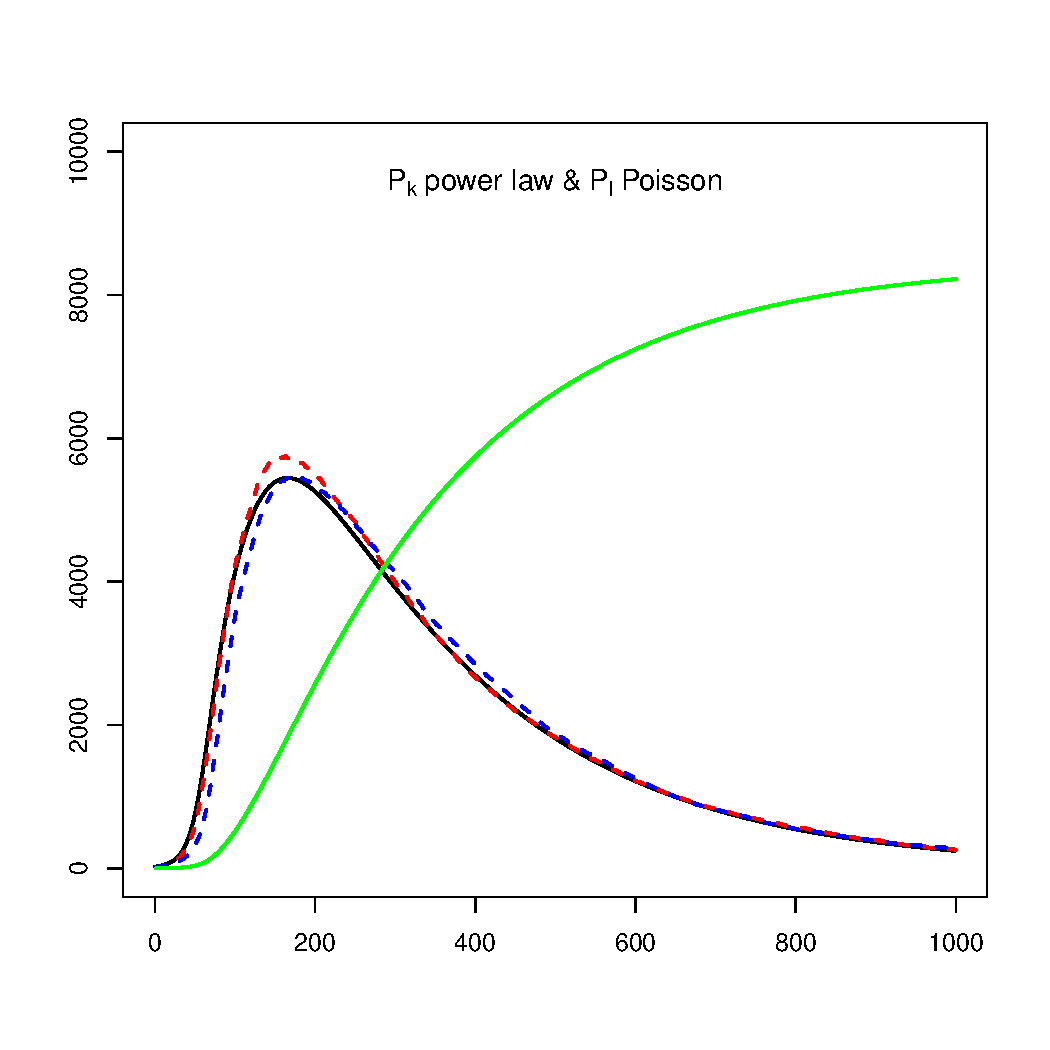
\includegraphics[width=\textwidth, trim=30 20 30 20, clip]{../img/sir_10.pdf}
    \end{subfigure}
    \newline
    \begin{subfigure}[b]{0.45\textwidth}
        \centering
        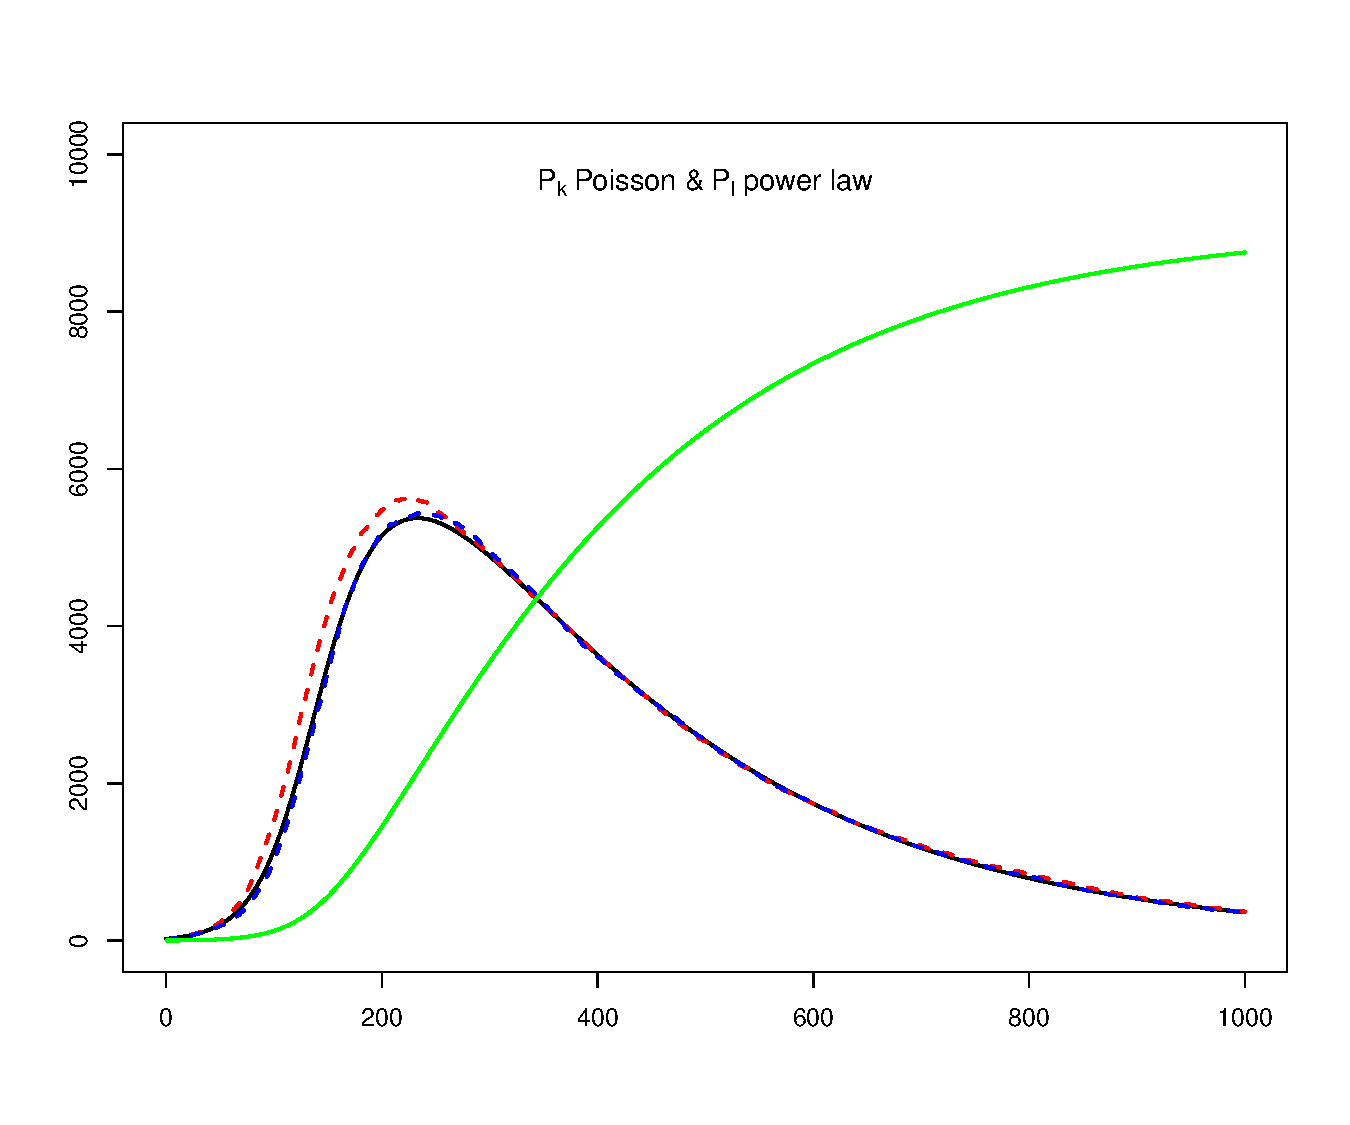
\includegraphics[width=\textwidth, trim=30 20 30 20, clip]{../img/sir_01.pdf}
    \end{subfigure}
    \hspace{0.08\textwidth}
    \begin{subfigure}[b]{0.45\textwidth}
        \centering
        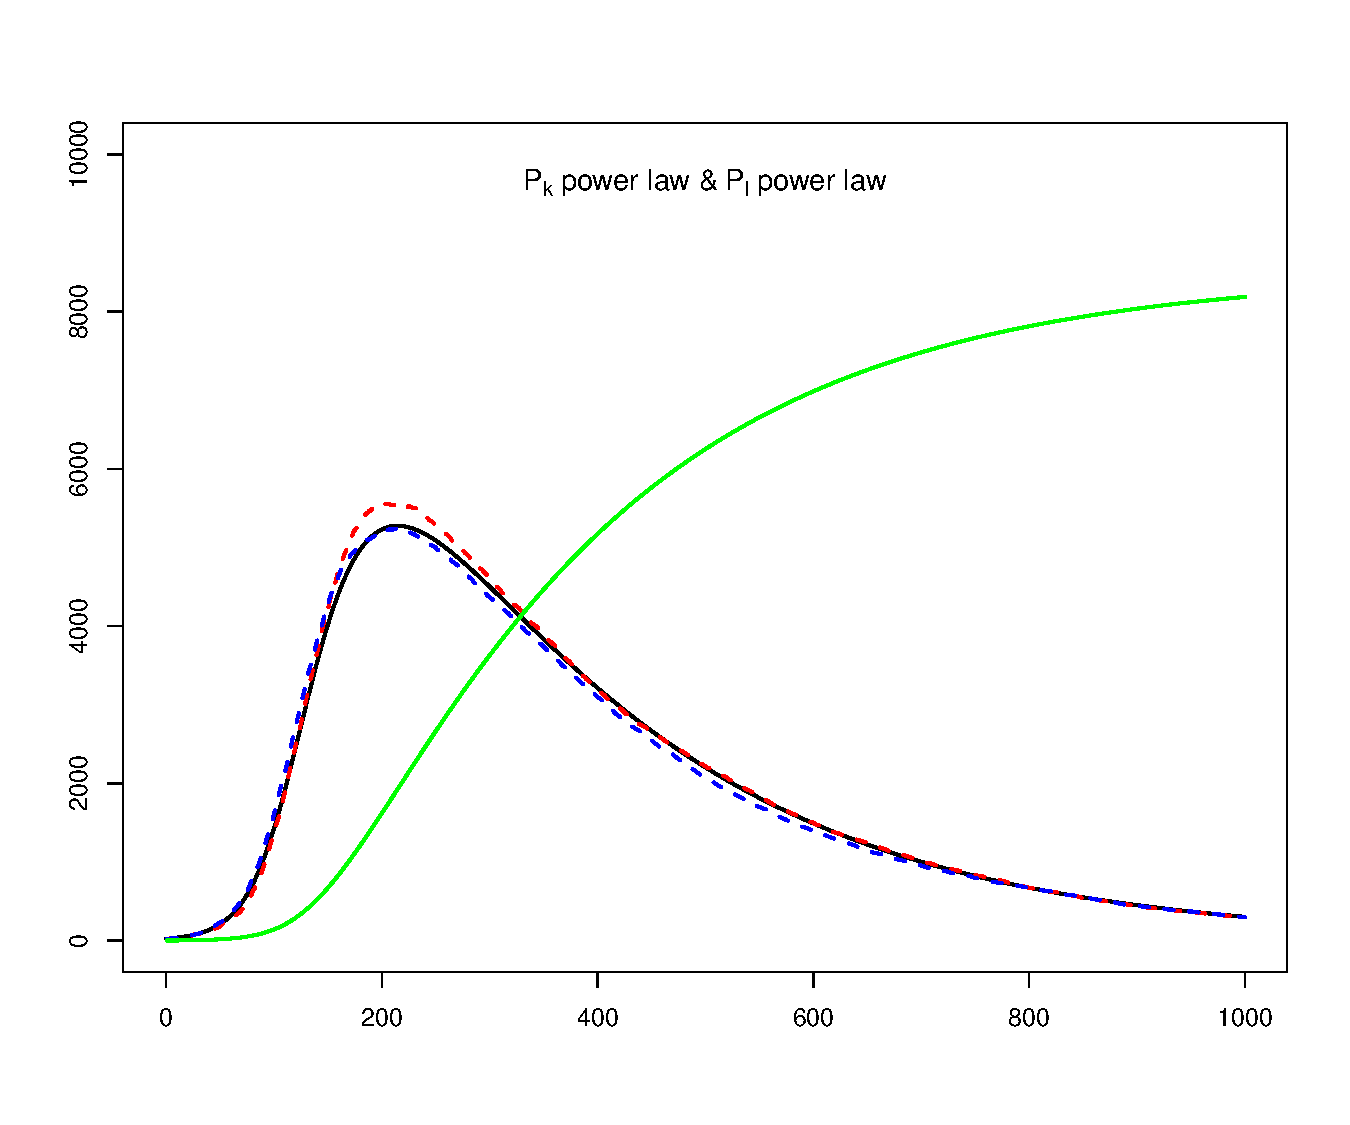
\includegraphics[width=\textwidth, trim=30 20 30 20, clip]{../img/sir_11.pdf}
    \end{subfigure}
    \newline
    \begin{subfigure}[b]{0.45\textwidth}
        \centering
        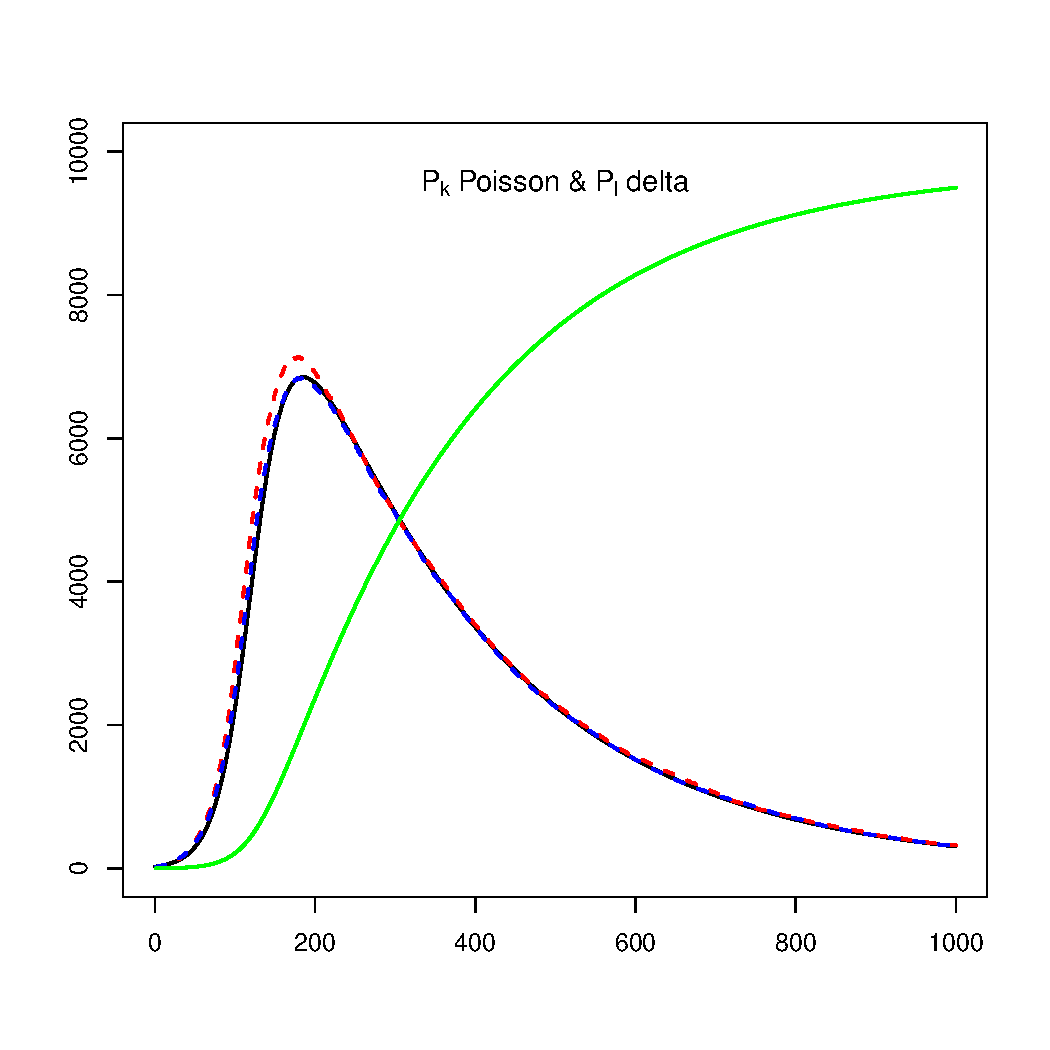
\includegraphics[width=\textwidth, trim=30 20 30 20, clip]{../img/sir_02.pdf}
    \end{subfigure}
    \hspace{0.08\textwidth}
    \begin{subfigure}[b]{0.45\textwidth}
        \centering
        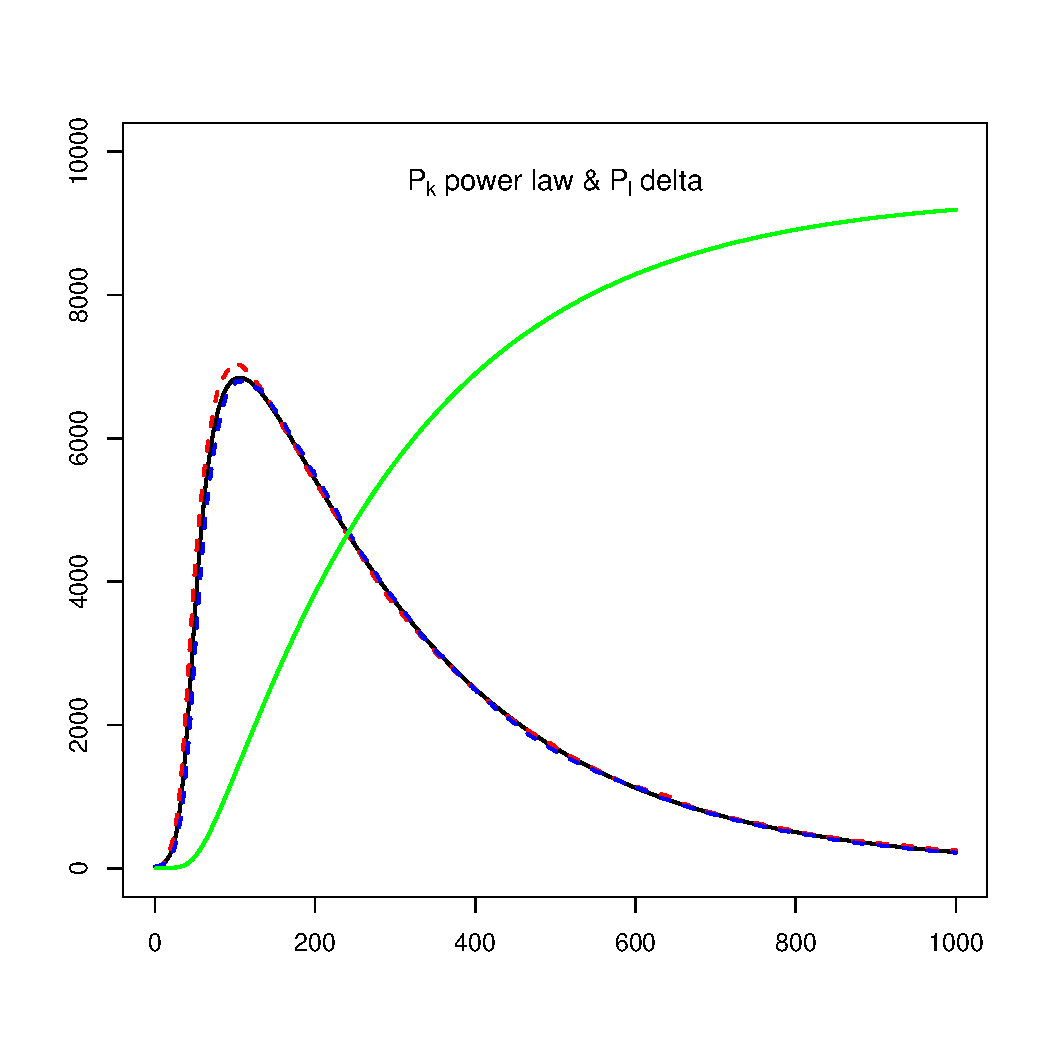
\includegraphics[width=\textwidth, trim=30 20 30 20, clip]{../img/sir_12.pdf}
    \end{subfigure}
    \newline
    \caption{Dynamics of the number of infected and recovered hosts during the SIR epidemic spreading on different types of networks.}
    \label{fig:sir_plots}
\end{figure*}

\begin{figure*}[hbtp]
    \centering
    \begin{subfigure}[b]{0.45\textwidth}
        \centering
          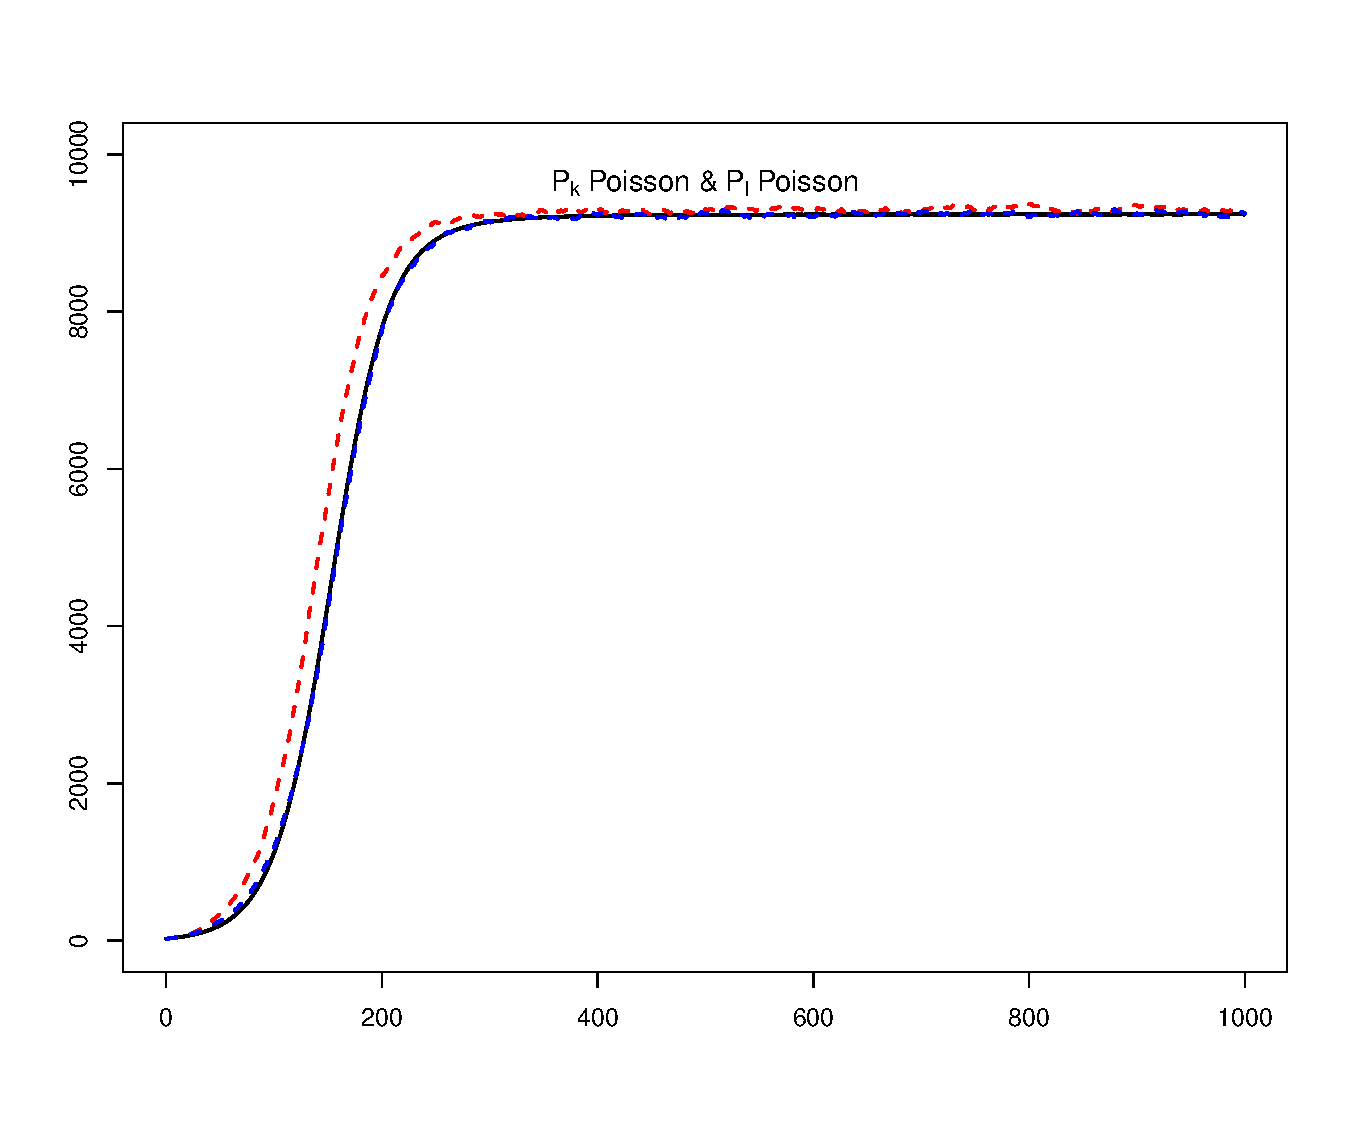
\includegraphics[width=\textwidth, trim=30 20 30 20, clip]{../img/sis_00.pdf}
    \end{subfigure}
    \hspace{0.08\textwidth}
    \begin{subfigure}[b]{0.45\textwidth}
        \centering
          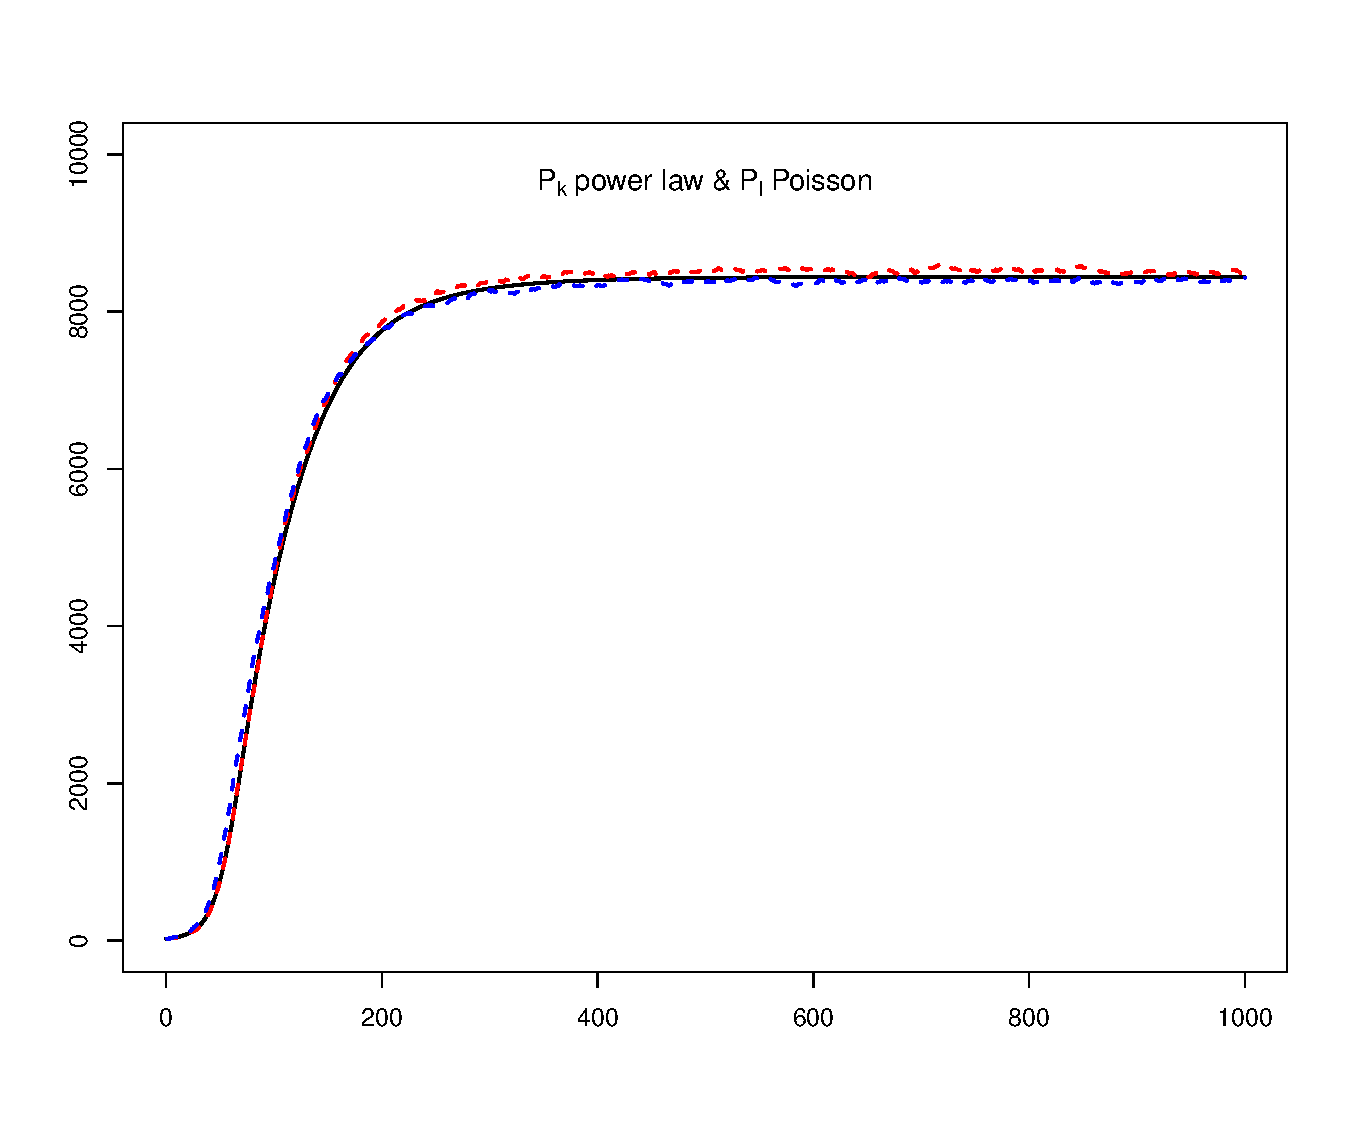
\includegraphics[width=\textwidth, trim=30 20 30 20, clip]{../img/sis_10.pdf}
    \end{subfigure}
    \newline
    \begin{subfigure}[b]{0.45\textwidth}
        \centering
        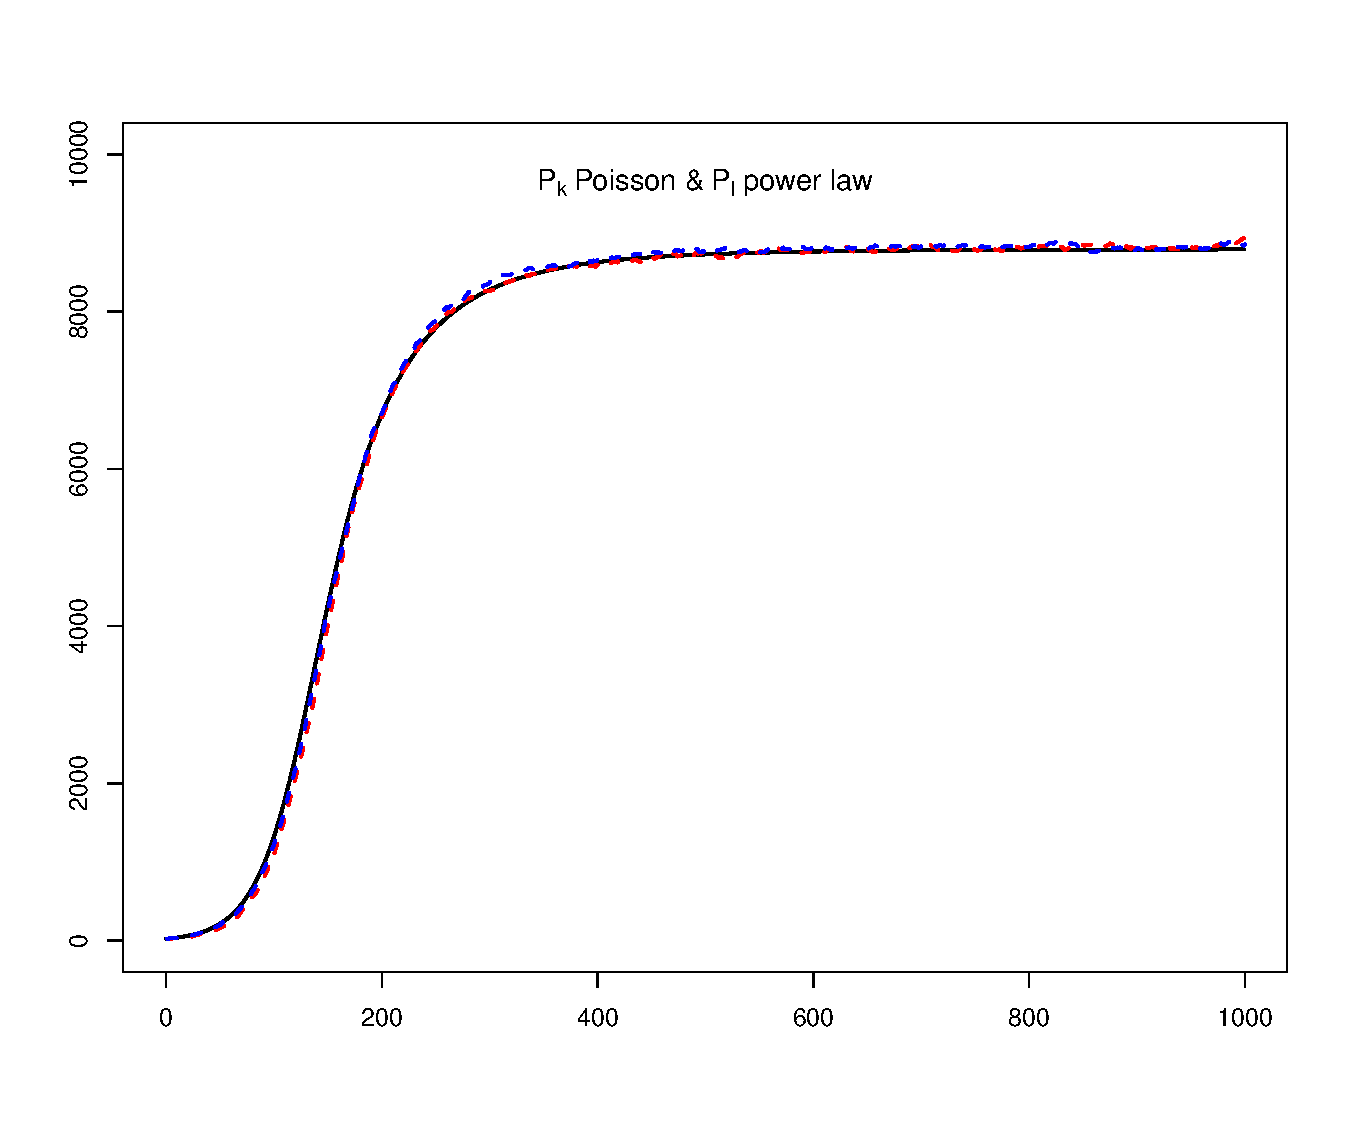
\includegraphics[width=\textwidth, trim=30 20 30 20, clip]{../img/sis_01.pdf}
    \end{subfigure}
    \hspace{0.08\textwidth}
    \begin{subfigure}[b]{0.45\textwidth}
        \centering
        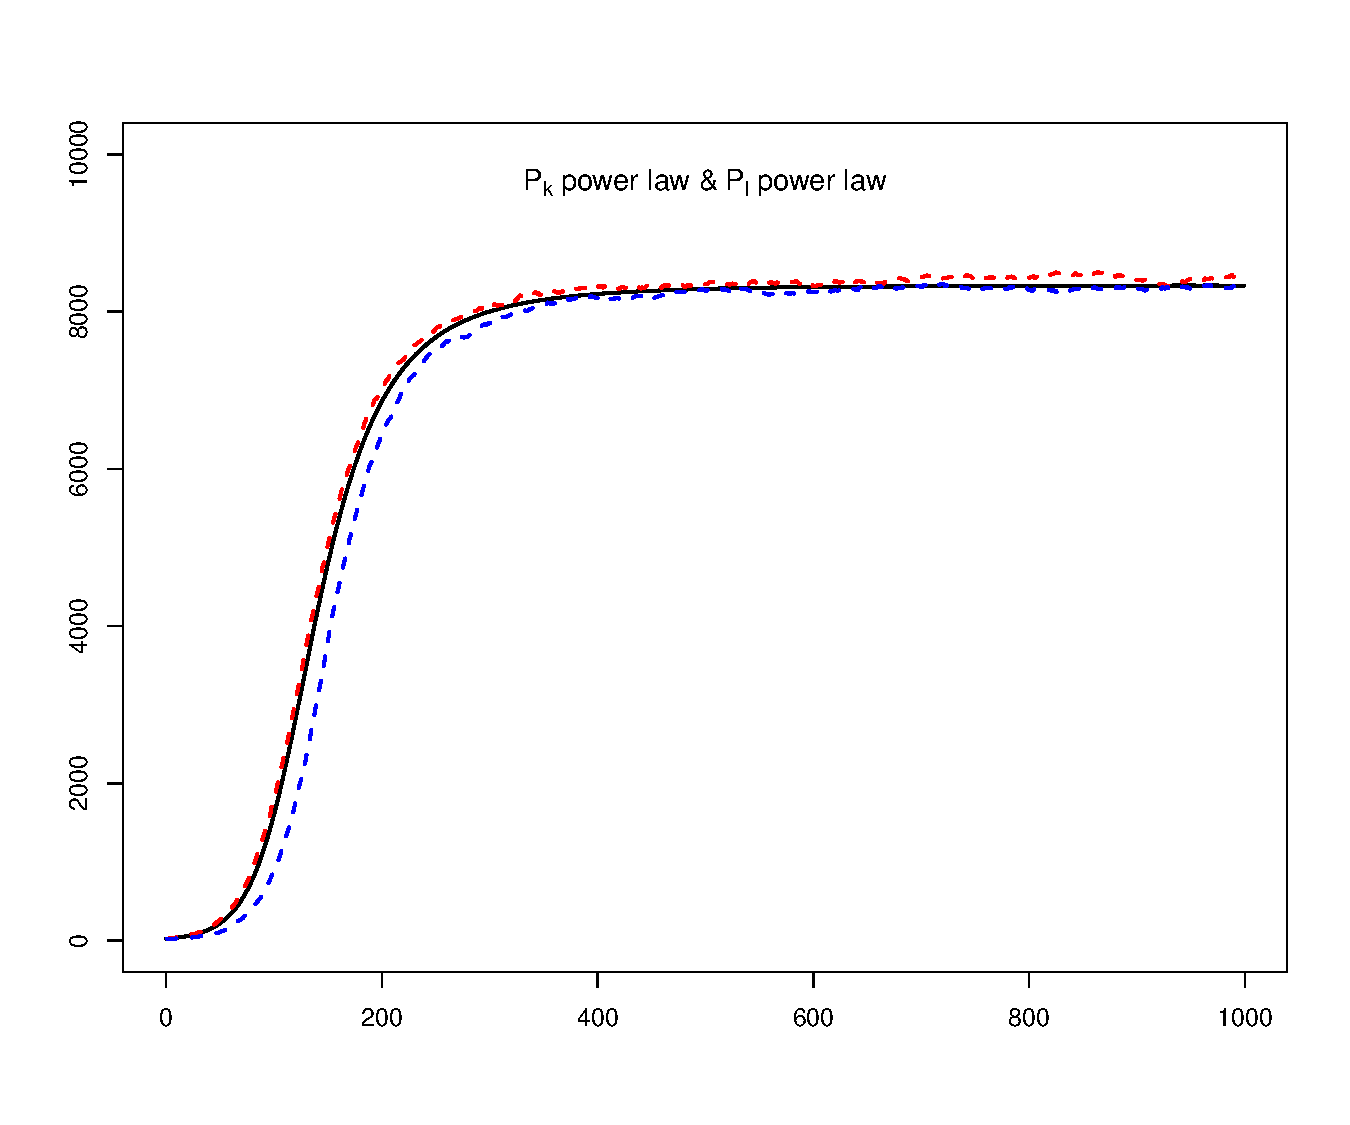
\includegraphics[width=\textwidth, trim=30 20 30 20, clip]{../img/sis_11.pdf}
    \end{subfigure}
    \newline
    \begin{subfigure}[b]{0.45\textwidth}
        \centering
        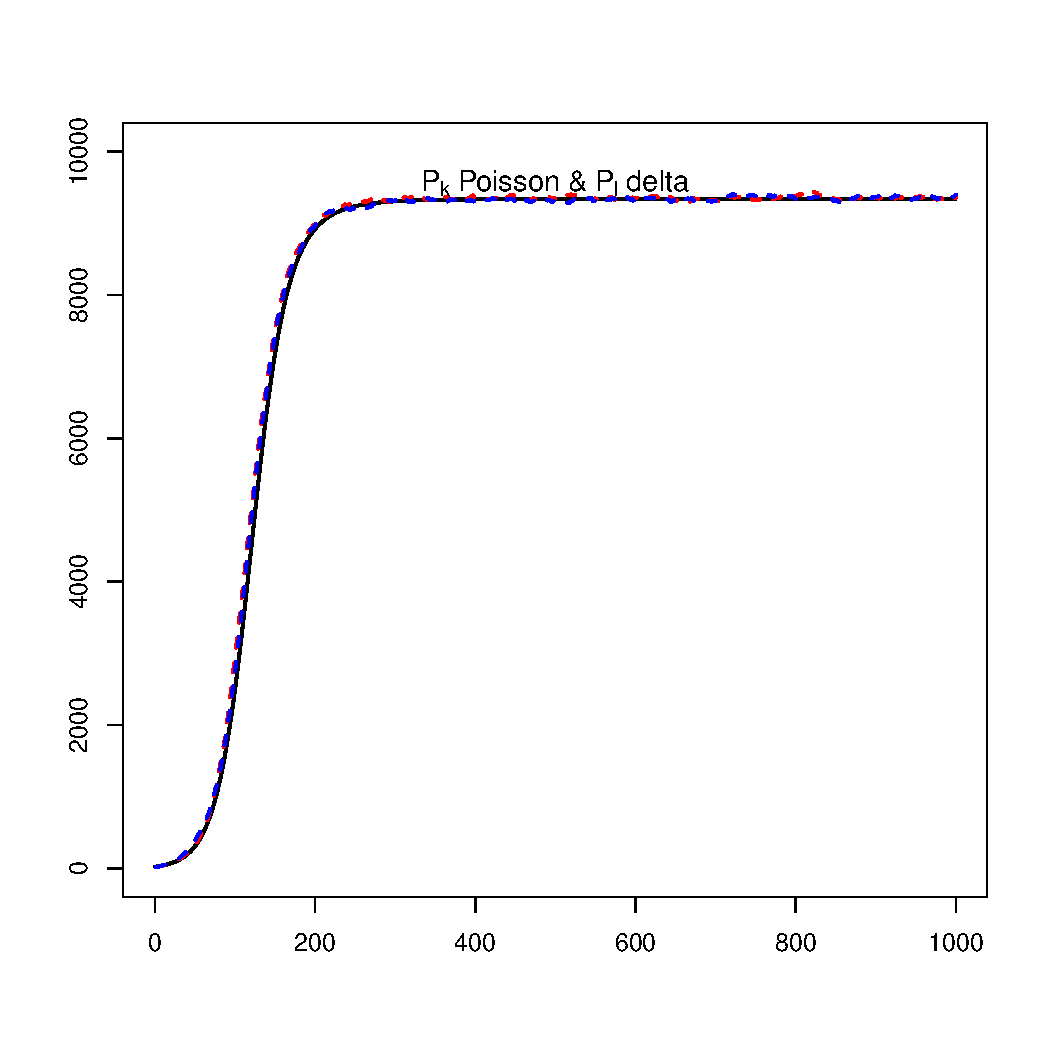
\includegraphics[width=\textwidth, trim=30 20 30 20, clip]{../img/sis_02.pdf}
    \end{subfigure}
    \hspace{0.08\textwidth}
    \begin{subfigure}[b]{0.45\textwidth}
        \centering
        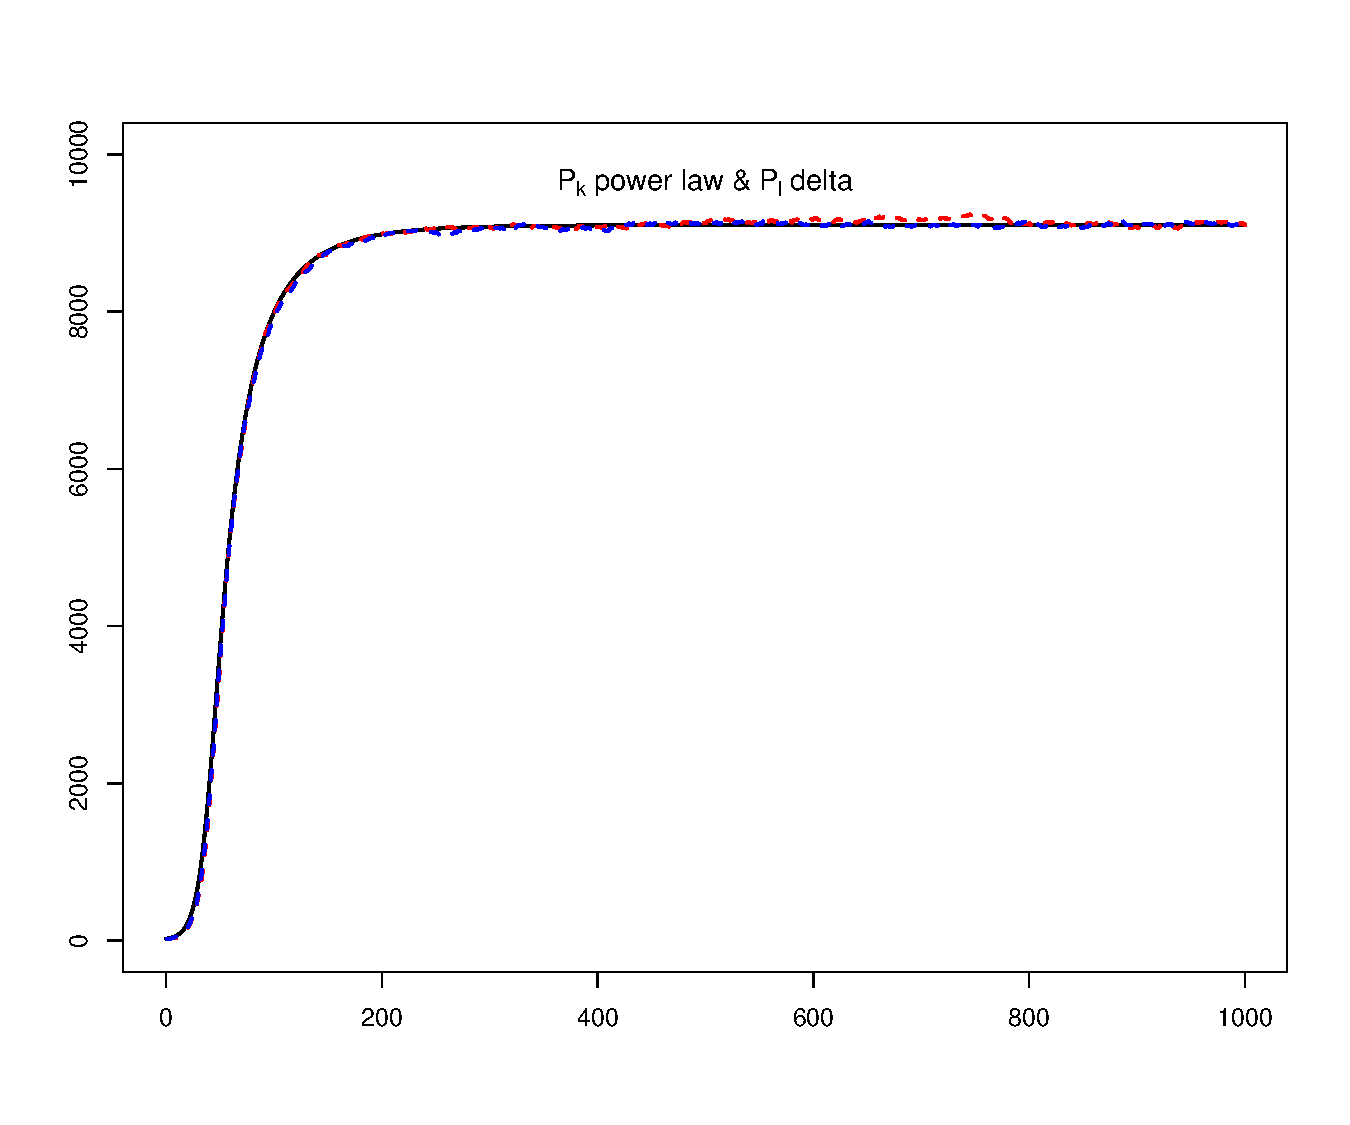
\includegraphics[width=\textwidth, trim=30 20 30 20, clip]{../img/sis_12.pdf}
    \end{subfigure}
    \newline
    \caption{Dynamics of the number of infected hosts during the SIS epidemic spreading on different types of networks.}
    \label{fig:sis_plots}
\end{figure*}